%! TeX program = lualatex
% use lualatex as primary compiler
\documentclass{beamer}

% Selects the theme defined in `beamerthemeUW.sty`
\usetheme{UW}

\usepackage{packages}
\usepackage{macros}
\usepackage{tcolorbox}
\usepackage{adjustbox}
\usepackage{graphicx}
\usepackage{bbm}
\usepackage{xcolor}
\usepackage{caption}



\title[RSLDS]{\small Bayesian Learning and Inference \\ in Recurrent Switching Linear Dynamical Systems}
%\subtitle{Subtitle}
%\author{Jane Doe\inst{1} \and John Doe\inst{2}}
\author{Charbel Abi Younes, Marvyn Bailly, Bart Boom, Rohin Gilman, Daran Xu}
\department{Applied Mathematics}
\date{May 1, 2023}
%\institute{
%    \inst{1}Very Fancy University \\
%    \inst{2}Another Fancy University
%}


\begin{document}

% The title slide
\begin{frame}
    \maketitle
\end{frame}

\begin{comment}
% The TOC
\begin{frame}{Table of Contents}
    \setcounter{framenumber}{1} % Sets the TOC to be the first numbered frame
    \tableofcontents
\end{frame}
\end{comment}

\section{Introduction and Motivation}

\begin{frame}{Introduction and Motivation}
        \begin{figure}[h!]
            \centering
            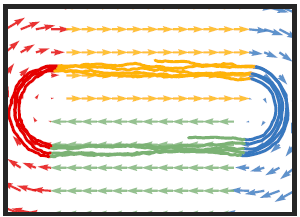
\includegraphics[width=0.6\textwidth]{fig1.png}
            \caption{NASCAR Dynamical System}
        \end{figure}

    \end{frame}

\section{Model}

\begin{frame}{Model}%{SLDS and rSLDS}

\begin{tcolorbox}[colback=blue!10!white,colframe=blue!50!black,title=SLDS and rSLDS,boxrule=2pt, boxsep=0.1em, left=0.1em, right=0.1em,
fontupper=\fontsize{8}{10}\selectfont] %,height=2in
\begin{enumerate}[\textbullet]
\item Continous latent state $x_{t+1}=A_{z_{t+1}}x_t+b_{z_{t+1}}+\nu_t \text{, } \nu_t \overset{\mathrm{iid}}{\sim} \mathcal{N}(0,Q_{z_{t+1}})$
\item Observation $y_t=C x_t+d+w_t\text{, }w_t \overset{\mathrm{iid}}{\sim} \mathcal{N}(0,S)$
    \item Discrete latent state $z_t \in \{1,\dots,K\}$
        \begin{itemize}
            \item SLDS {\cite{Ackerson&Fu}}
$z_{t+1} | z_t \sim \pi_{z_t}$
            \item rSLDS {\cite{Barber}}
 $z_{t+1} | z_t, x_t \sim \pi_{SB}(\nu_{t+1})$, $\nu_{t+1}=R_{z_t}x_t+r_{z_t}$
        \end{itemize}
\end{enumerate}
\end{tcolorbox}
       

%\begin{figure}
    %\centering
    %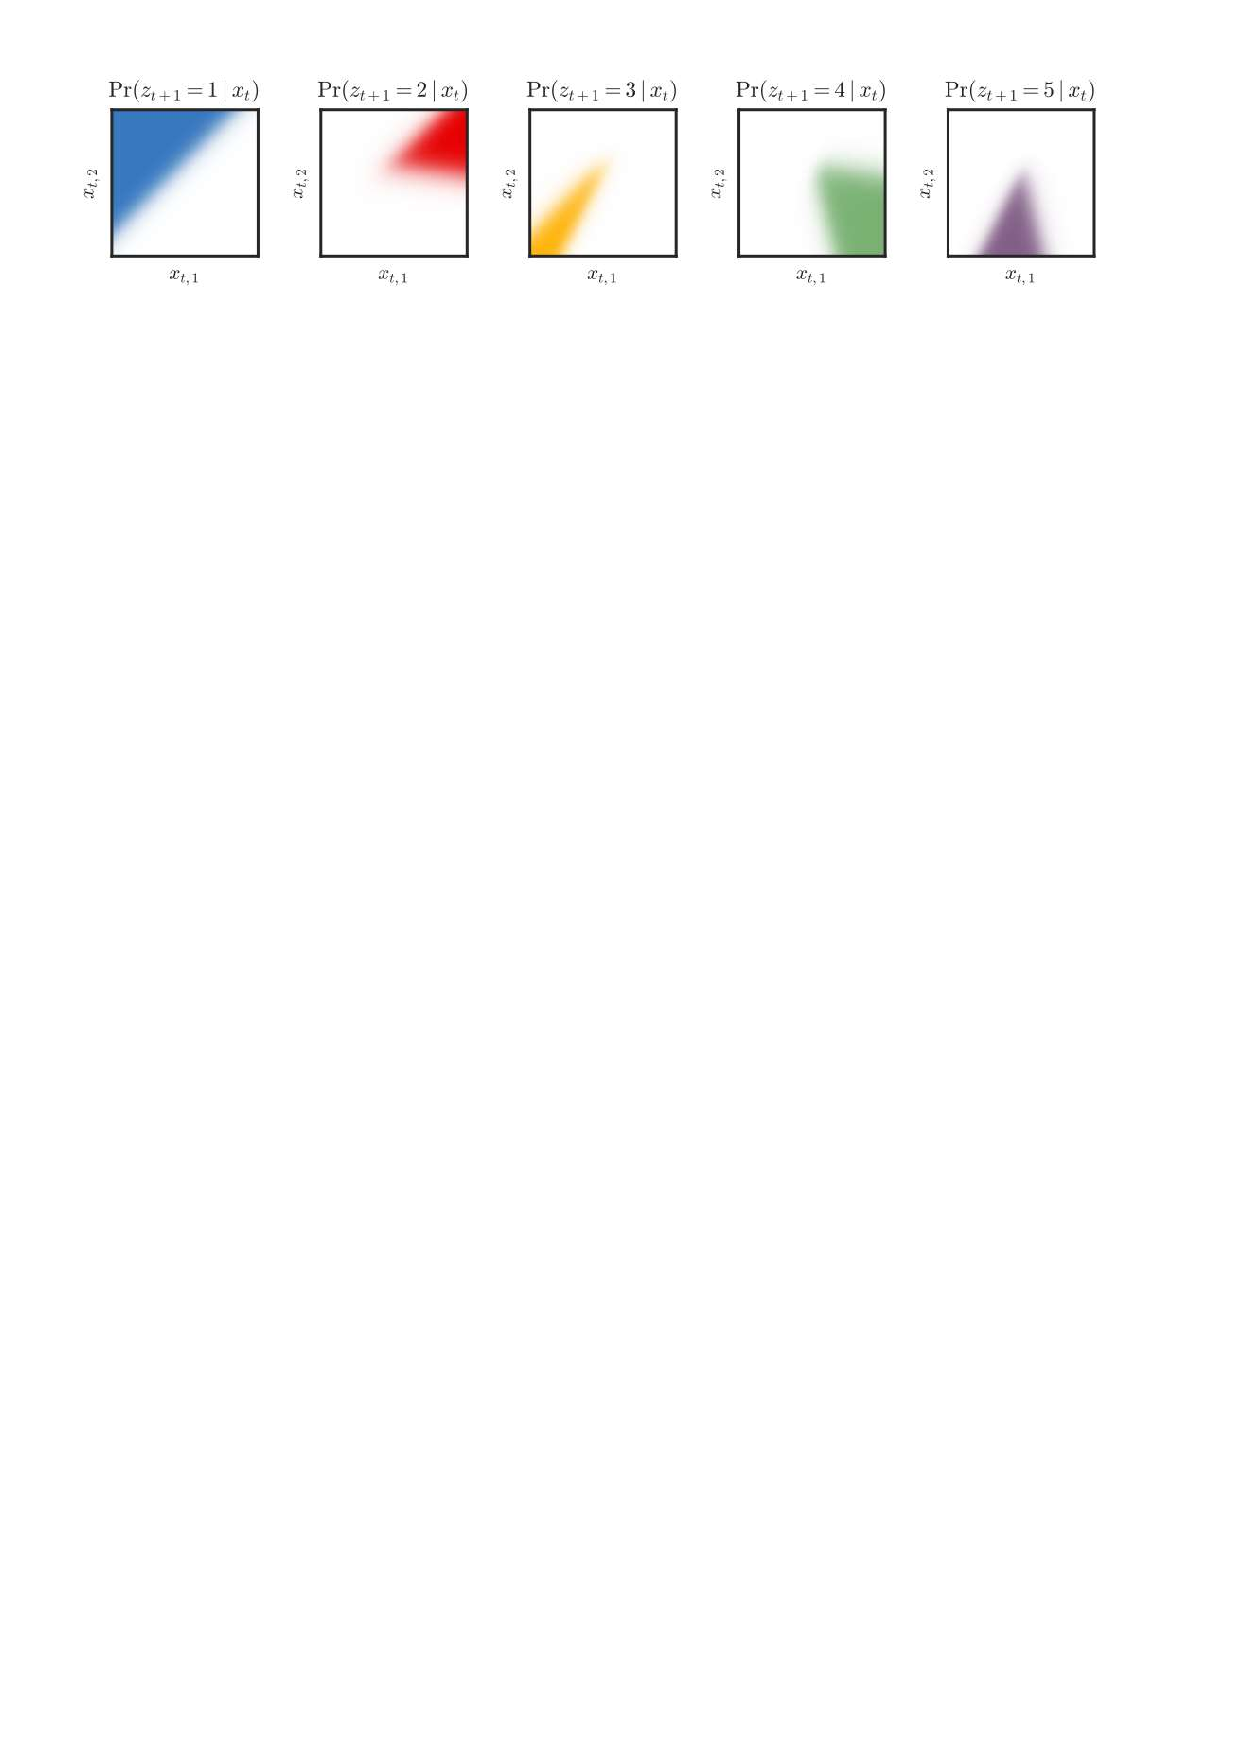
\includegraphics[width=1.2\linewidth]{gallery/z_on_x.pdf}
    %\caption{}
 % \end{figure}
   

\begin{figure}
    %\captionsetup{position=top}
	\centering
    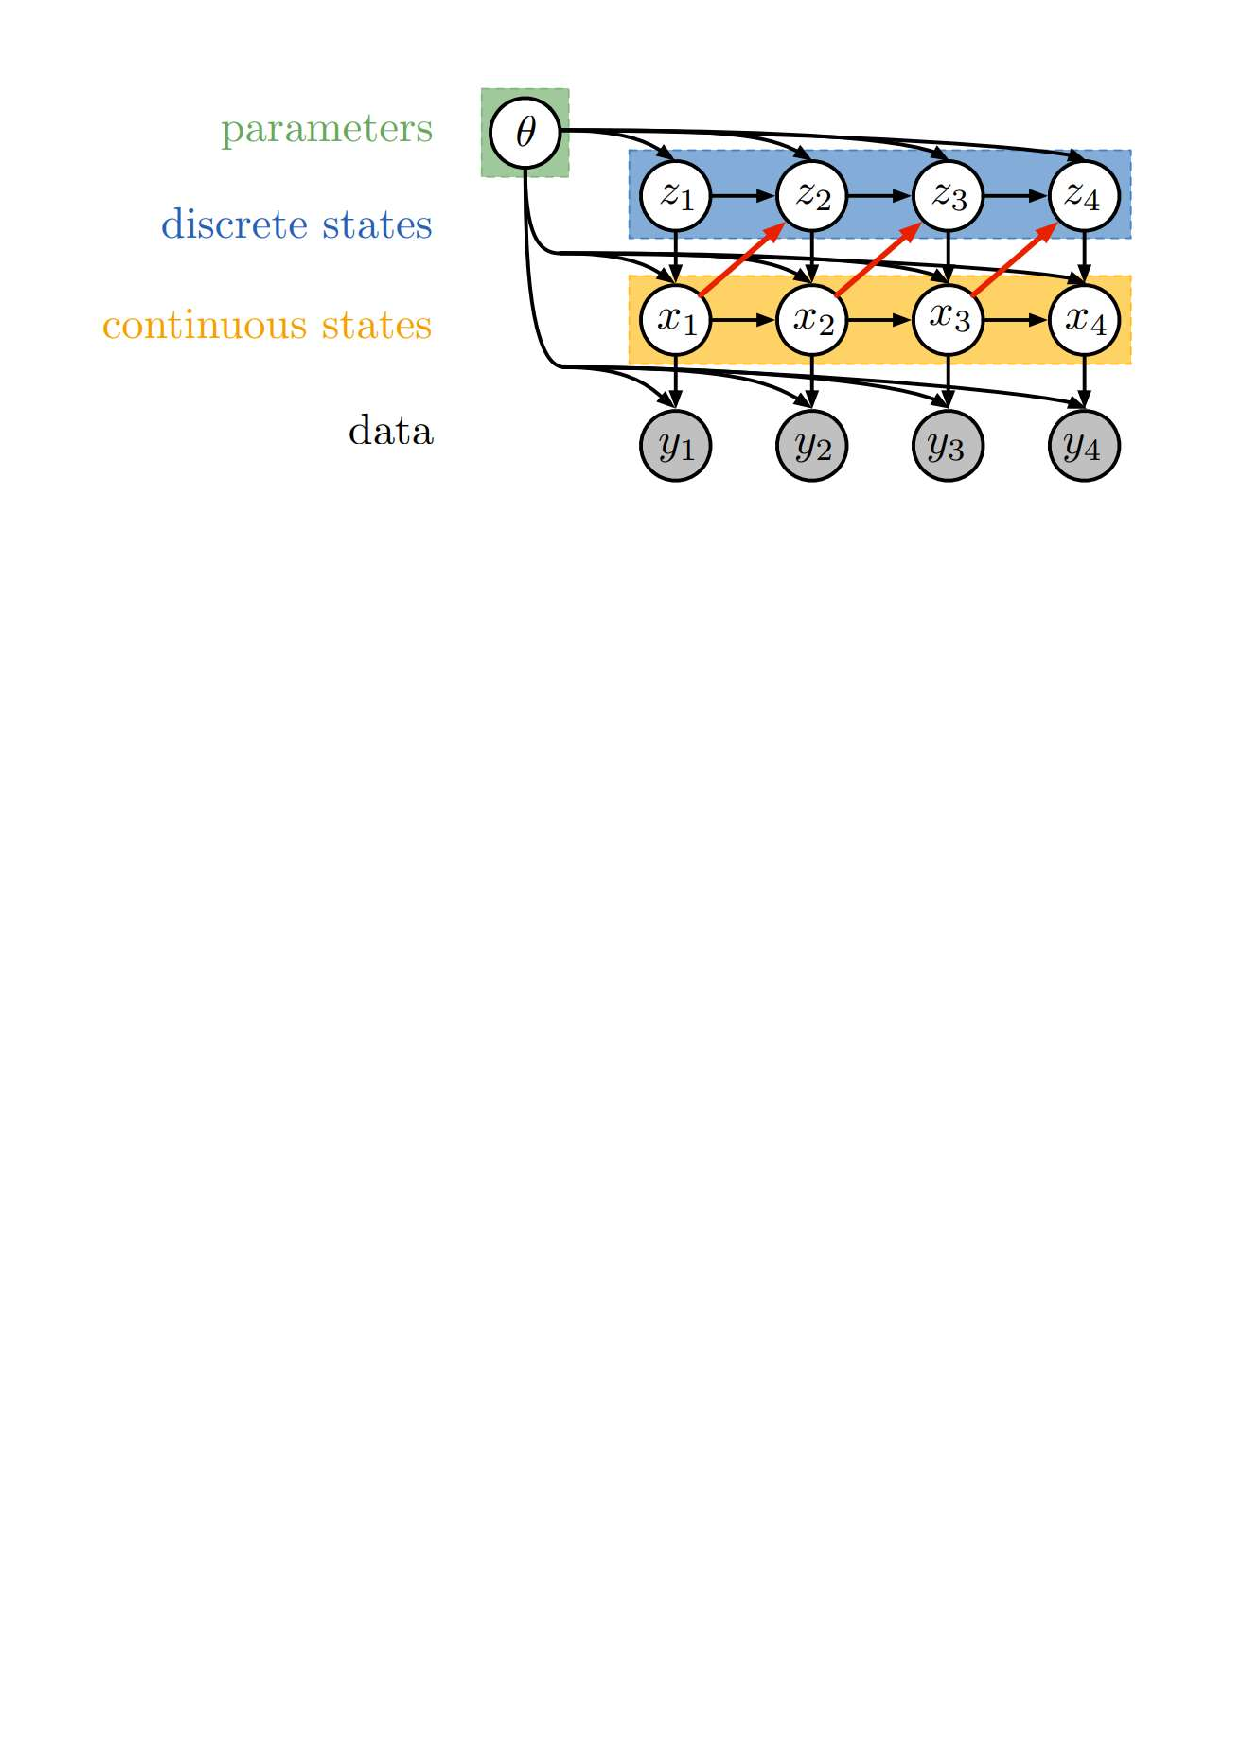
\includegraphics[width=1.0\linewidth]{gallery/rSLDS.pdf}
	%\caption{$z_t \in \{1,2,3,4,5\}, x_t \in \mathbb{R}^2$}
\end{figure}


%\begin{figure}
%    \centering
%    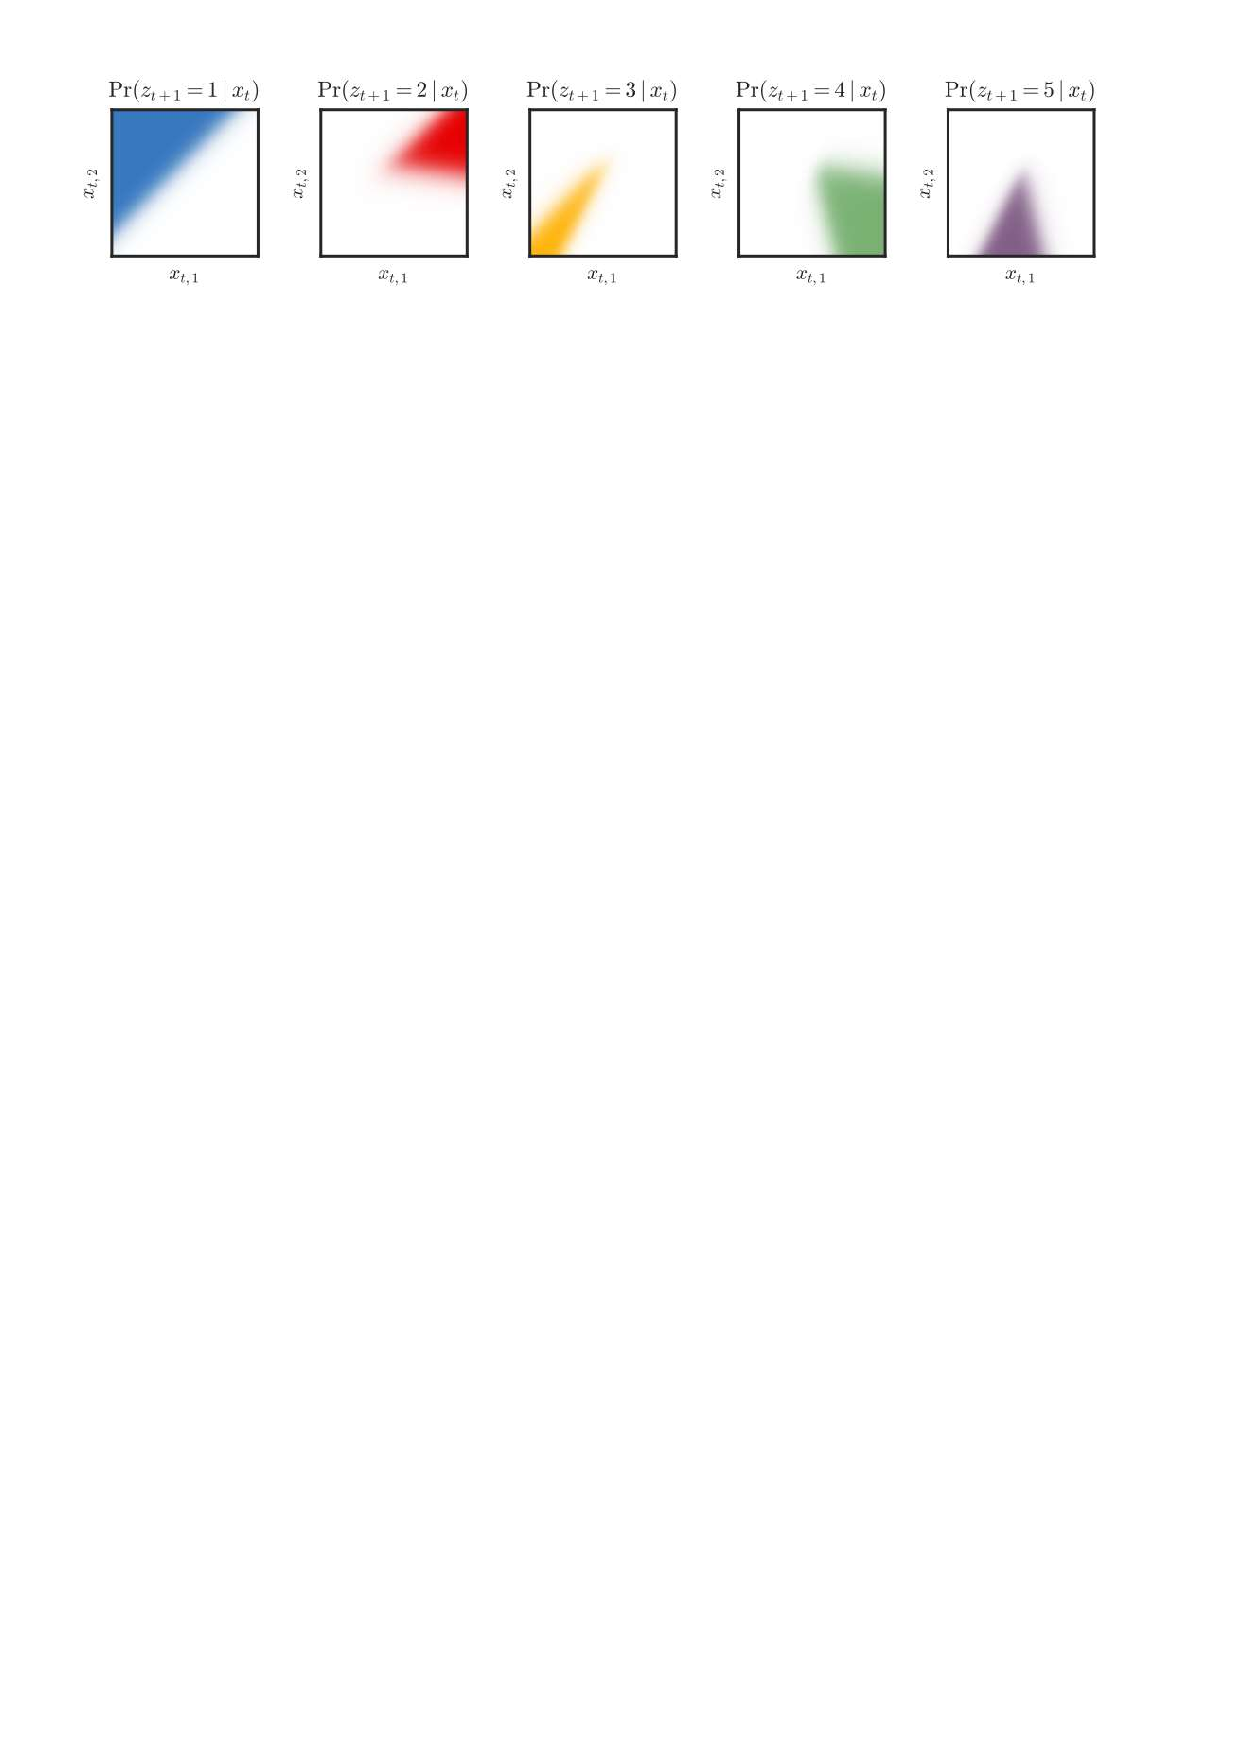
\includegraphics[scale=0.3]{gallery/z_on_x.pdf}
%    \caption{Dependence of $z_{t+1}$ on $x_t$}
%    \label{rLSDS}
%\end{figure}
%\begin{figure}
%    \centering
%    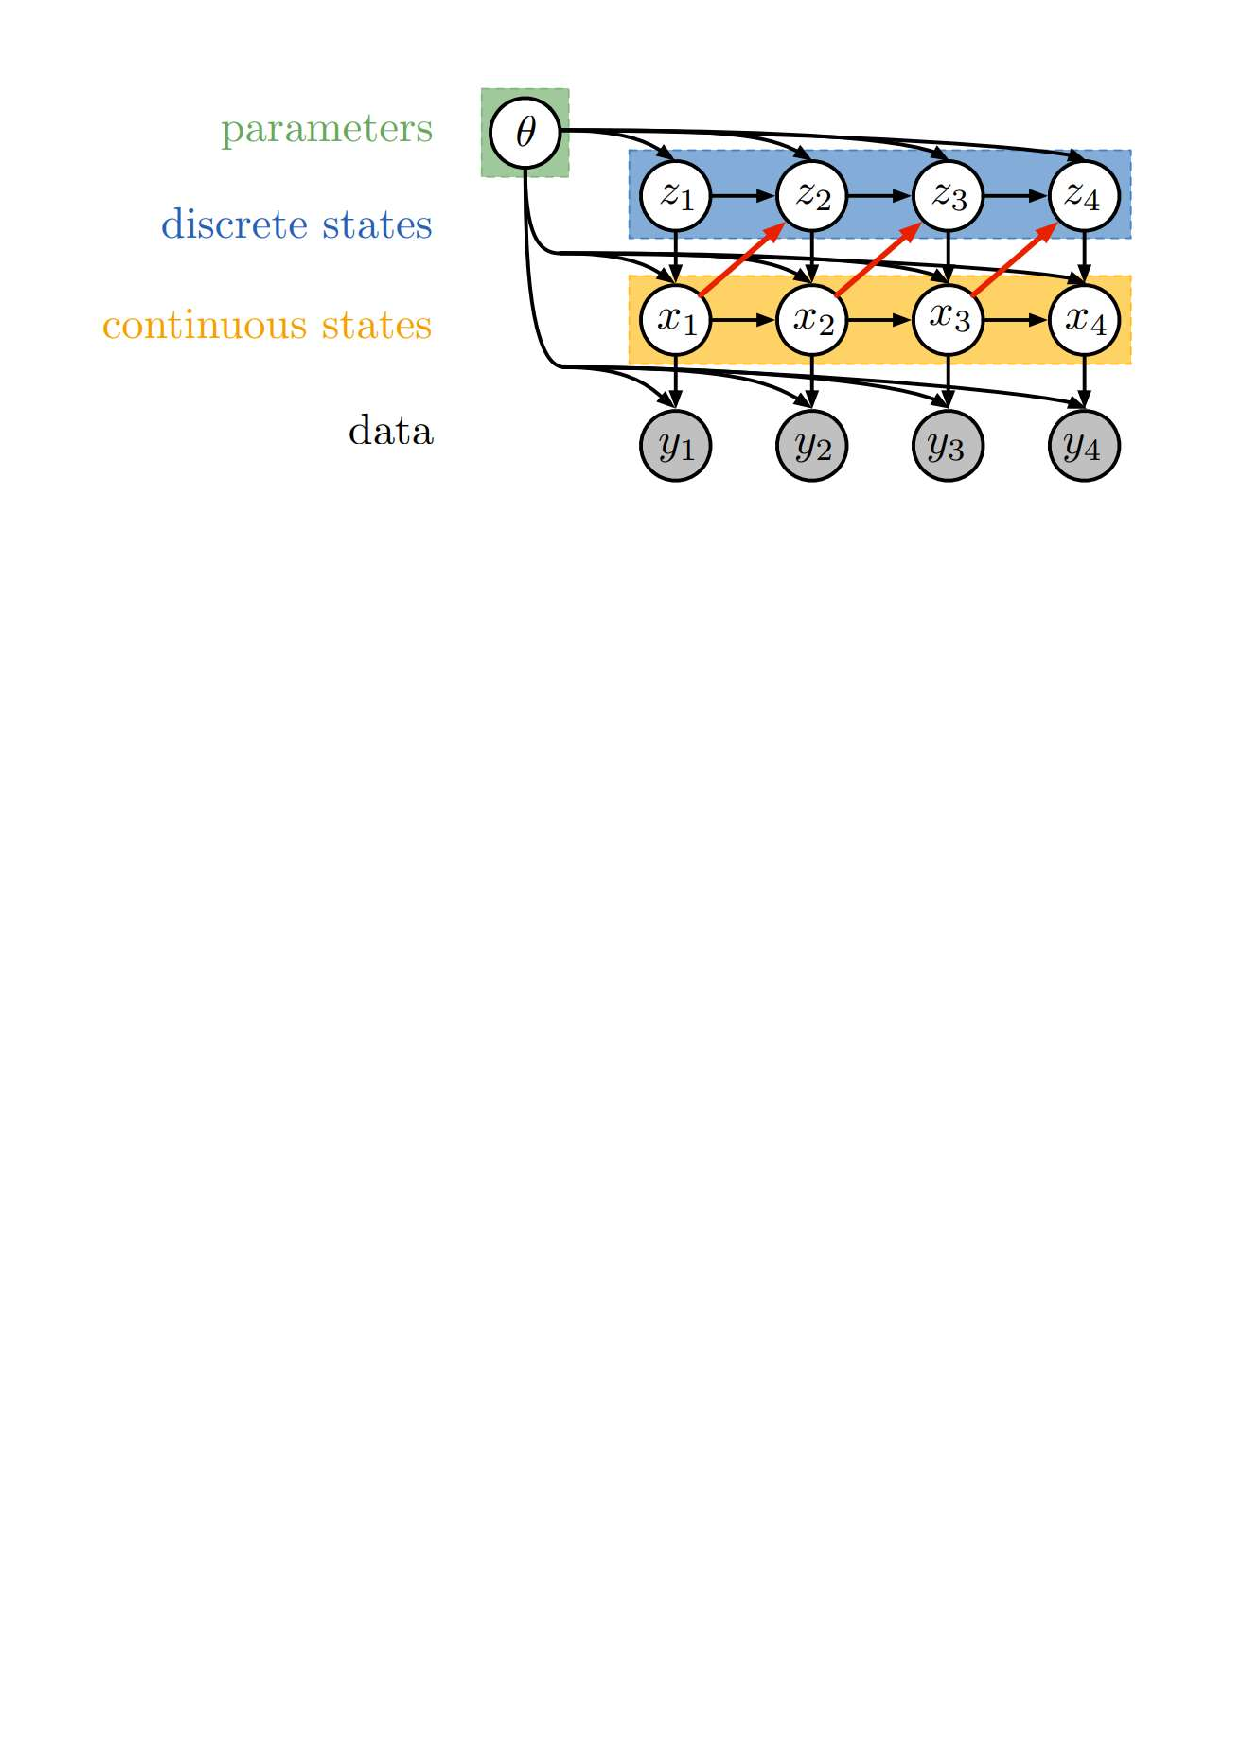
\includegraphics[scale=0.3]{gallery/rSLDS.pdf}
%    \caption{Graphical Model for the rSLDS}
%    \label{rLSDS}
%\end{figure}

    \end{frame}

\begin{frame}{Model}%{Stick Breaking Logitstic Regression}
       \begin{tcolorbox}[colback=blue!10!white,colframe=blue!50!black,title=Stick Breaking Logitstic Regression \cite{linderman2015dependent},boxrule=2pt, boxsep=0.1em, left=0.1em, right=0.1em,
fontupper=\fontsize{8}{10}\selectfont] %,height=2in
\begin{enumerate}[\textbullet]

\item $p(z|x) \sim \pi_{SB}(\nu),\text{ } \nu=Rx+r$
\item Link function: $\pi_{SB}(\nu)=\left( \pi_{SB}^{(1)}(\nu),\dots,\pi_{SB}^{(K)}(\nu) \right)$ (with $\sigma(x)=\frac{e^x}{1+e^x}$)\\
%\sigma(\nu_k) \prod_{j<k}\left(1- \sigma(\nu_j)\right)=
$\pi_{SB}^{(k)}(\nu)=\begin{cases}
    \sigma(\nu_k) \prod_{j<k}\sigma(-\nu_j),& \text{if } k=1,\dots,K-1\\
    \prod_{1}^K \sigma(-\nu_j),              & \text{if} k=K
\end{cases}$\\

\item 
$p(z|x) \sim \prod _{k=1}^K \sigma(\nu_k)^{\mathbbm{1} [z=k]} \sigma(-\nu_k)^{\mathbbm{1} [z>k]}$ (Likelihood)
\end{enumerate}
\end{tcolorbox}
\begin{enumerate}[\textbullet]
\item With a Gaussian Prior $p(x)$, the posterior $p(x|z)\propto p(x)*p(z|x)$ is non-Gaussian
\item Bayesian updating is not efficient
\begin{itemize}
            \item Gibbs Sampler: sampling $x^{(i+1)} \sim p(x|z=z^{(i)})$, sampling $z^{(i+1)} \sim p(z|x=x^{(i+1)})$			

%            \item Message Passing
%$m_{t \rightarrow \left(t+1\right)}(x_{t+1})=\int \psi\left(x_{t}, y_{t}\right) \textcolor{blue}{\psi\left(x_{t}, z_{t+1}\right)} \psi\left(x_{t}, x_{t+1}, z_{t+1}\right) m_{\left(t-1\right) \rightarrow t}\left(x_{t}\right) \mathrm{d} x_{t}$

\end{itemize}
\end{enumerate}


    \end{frame}

\begin{frame}{Model}%{Inference}
        \begin{tcolorbox}[colback=blue!10!white,colframe=blue!50!black,title=Polya-gamma augmentation\cite{linderman2015dependent},boxrule=2pt, boxsep=0.1em, left=0.1em, right=0.1em,
fontupper=\fontsize{8}{10}\selectfont]

\begin{align}
\textcolor{blue}{ \frac{\left(e^{\nu}\right)^{a}}{\left(1+e^{\nu}\right)^{b}} } &=2^{-b}  \int_{0}^{\infty} \boldsymbol{e^{\kappa \nu} e^{-\omega \nu^{2} / 2} }\textcolor{red} {  p_{\text {PG }}(\omega \mid b, 0) }\mathrm{d} \omega \text{ }(\kappa=a-\frac{b}{2})\\
p(x_{t}|z_{t+1}) &\propto \prod_{k=1}^{K-1} \textcolor{blue}{  \frac{\left(e^{\nu_{t+1, k}}\right)^{\mathbb{I}\left[z_{t+1}=k\right]}}{\left(1+e^{\nu_{t+1, k}}\right)^{\mathbb{I}\left[z_{t+1} \geq k\right]}} }\\
p(x_t|z_{t+1})&=\int p(x_t,\omega_t|z_{t+1})  \mathrm{d}\omega_t=\int   \boldsymbol{ p(x_t|z_{t+1},\omega_t) }\textcolor{red}{ p(\omega_t) } \mathrm{d}\omega_t  \\
\omega_{t, k} \mid x_{t}, z_{t+1} &\sim \operatorname{PG}\left(\mathbb{I}\left[z_{t+1} \geq k\right], \nu_{t+1, k}\right) 
\end{align}

\end{tcolorbox}
\begin{itemize}
\item $p(x_t|z_{t+1},\omega_t)$ is Gaussian 
%\item Message Passing $\psi(x_t,z_{t+1},\omega_t) \propto \mathcal{N}(\nu_{t+1}|\Omega^{-1}_t \kappa_{t+1},\Omega^{-1}_t)$
\item Thus instantiating these auxiliary variables in a Gibbs
sampler enables efficient block updates
\end{itemize}

    \end{frame}


\section{Conclusion}

\begin{frame}{Conclusions}
        \begin{itemize}
            \item SLDS vs rSLDS
            \begin{figure}[h!]
                \centering
                \begin{subfigure}[b]{0.3\textwidth}
                    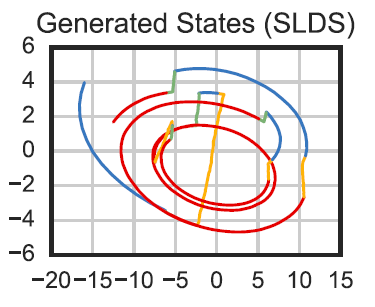
\includegraphics[width=\textwidth]{fig2.png}
                \end{subfigure}
                \begin{subfigure}[b]{0.3\textwidth}
                    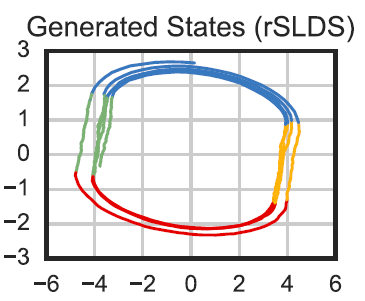
\includegraphics[width=\textwidth]{fig3.png}
                \end{subfigure}
            \end{figure}

            \item Canonical Dynamical System - Lorenz Attractor
            \begin{figure}[h!]
                \centering
                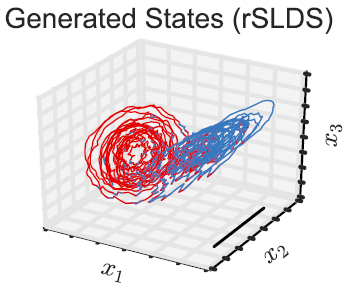
\includegraphics[width=0.3\textwidth]{fig4.png}
            \end{figure}
        \end{itemize}

    \end{frame}

\section{Next Step}

\begin{frame}{Next Steps}
        \begin{itemize}
            \item Van der Pol Oscillator
            \begin{itemize}
                \item Canonical dynamical system with a stable limit cycle and bifurcations
            \end{itemize}

            \vspace{2em}

            \item Double Pendulum
            \begin{itemize}
                \item System with chaotic dynamics and multiple states (depending on the relative positions of the weights)
            \end{itemize}

        \end{itemize}

    \end{frame}
\begin{comment}
\subsection{A Subsection}

    \begin{frame}{Frame Title}{Frame Subtitle}
        This is a frame with a title and a subtitle.

    \end{frame}

    \begin{frame}{\null}
        This is a frame with no title.
    \end{frame}

    \begin{frame}
        This is a frame with no header.
    \end{frame}

\subsection{Another Subsection}

    \begin{frame}{Text}
        \underline{This is underlined text.}

        \textit{This is italic text.}

        \textbf{This is bold text.}

        \texttt{This is mono-spaced text.}
    \end{frame}

    \begin{frame}{Lists}
        This is a bulleted list:
        \begin{itemize}
            \item An item

            \item Another item
            \begin{itemize}
                \item A subitem

                \item Another subitem
            \end{itemize}
        \end{itemize}

        This is a numbered list:
        \begin{enumerate}
            \item An item

            \item Another item
            \begin{enumerate}
                \item A subitem

                \item Another subitem
            \end{enumerate}
        \end{enumerate}
    \end{frame}

    \begin{frame}{Colored Blocks}
        \begin{block}{Block Title}
            This is a block.
        \end{block}

        \begin{alertblock}{Alert Block Title}
            This is an alertblock.
        \end{alertblock}

        \begin{example}
            This is an example block.
        \end{example}
    \end{frame}


%~~~~~~~~~~~~~~~~~~~~~~~~~~~~~~~~~~~~~~~~~~~~~~~~~%


\section{Second Section}

    \begin{frame}{Frame Title}
        This is a frame the second section.
    \end{frame}

    \begin{frame}{Frame Title}
        This is a frame with a...

        \pause

        \texttt{\textbackslash pause}.
    \end{frame}
\end{comment}

\section{Bibliography}

    \nocite{Ackerson&Fu}
    \nocite{Barber}
	\nocite{linderman2015dependent}


    \begin{frame}{Bibliography}
        \bibliographystyle{plain}
        \bibliography{bibliography_file}
    \end{frame}

\end{document}
